\documentclass[conference]{IEEEtran}
\IEEEoverridecommandlockouts

\usepackage{fancyhdr}
\pagestyle{fancy}
\fancyhf{}

\renewcommand{\thepage}{\Roman{page}} % Capital Roman numerals

\fancyhead[L]{\thepage}                 % Page number on left
\fancyhead[C]{A. SEN, S. VERMA, S. TULSYAN \& S. DHANUKA}

\usepackage{cite}
\usepackage{amsmath,amssymb,amsfonts}
\usepackage{algorithmic}
\usepackage{graphicx}
\usepackage{textcomp}
\usepackage{xcolor}
\usepackage{booktabs}
\usepackage{multirow}

\newcommand{\Var}{\mathrm{Var}}
\newcommand{\R}{\mathbb{R}}

\begin{document}

\title{Quantitative Analysis of Media Bias and Stock Price Dynamics: The 2020 Shock}

\author{\small
\begin{minipage}[t]{0.48\textwidth}
\centering
Anirban Sen \\
\textit{Dept of CS} \\
\textit{Ashoka University} \\
Sonipat, India \\
anirban.sen@ashoka.edu.in
\end{minipage}
\hfill
\begin{minipage}[t]{0.48\textwidth}
\centering
Shivansh Verma \\
\textit{Dept of CS} \\
\textit{Ashoka University} \\
Sonipat, India \\
shivansh.verma\_ug2023@ashoka.edu.in
\end{minipage}
\\[0.6em]
\begin{minipage}[t]{0.48\textwidth}
\centering
Soham Tulsyan \\
\textit{Dept of CS} \\
\textit{Ashoka University} \\
Sonipat, India \\
soham.tulsyan\_ug2023@ashoka.edu.in
\end{minipage}
\hfill
\begin{minipage}[t]{0.48\textwidth}
\centering
Sashwat Dhanuka \\
\textit{Dept of CS} \\
\textit{Ashoka University} \\
Sonipat, India \\
sashwat.dhanuka\_ug2023@ashoka.edu.in
\end{minipage}
}

\maketitle

\thispagestyle{empty}

\begin{abstract}
This paper studies how media reporting about large-cap firms changed around the 2020 recession and whether shifts in news stance predict firm-level stock outcomes. Using a large-scale NewsMTSC pipeline to compute daily stance scores from full-text news articles (2015--2025) for S\&P 500 firms, we combine NLP-derived stance with firm-day controls and market variables to test structural shifts, causal responses, and predictive linkages. Our identification strategy centers on a pre/post shock design around January 2020, complemented by difference-in-differences, interrupted time series, and time-series VAR exercises. We document the data pipeline, relevance filtering, stance aggregation, and robustness checks used throughout the analysis.
\end{abstract}

\section{Introduction}
The 2020 recession is a natural breakpoint for studying the interaction between media narratives and financial markets. COVID-era coverage expanded in volume and intensity, and a growing body of evidence documents a structural change in news-market dynamics during and after the shock. This project asks a simple, high-level question: did the tone of firm-specific media reporting shift after 2020, and if it did, did markets respond differently to that tone?

We approach the problem with a target-dependent stance framework rather than generic sentiment. NewsMTSC allows us to score whether an article is positive or negative toward a specific firm even when multiple firms are mentioned in the same text. That distinction is central to firm-level testing: a general sentiment score cannot distinguish positive coverage of one firm from negative coverage of another in the same article. Target-dependent stance makes it feasible to construct a daily, firm-level media stance signal and evaluate how it behaves across time and shocks.

The study is grounded in three observations from the project work so far. First, the 2020 shock is widely documented as a period in which media coverage and market behavior changed in a persistent way. Second, the data pipeline needs to be precise: naive keyword search introduces many false positives and inflates noise in the stance signal. Third, if stance is to be linked to returns in a credible way, the design must rule out coverage volume effects, pre-trend differences, and spurious correlations driven by macro shocks.

We therefore build a two-stage pipeline: (i) relevance classification that filters articles to those that actually report on the target firm, and (ii) NewsMTSC stance scoring with confidence thresholds. With this signal we pose three research questions on structural shifts in stance and returns and the post-shock stance-return linkage. Our empirical strategy combines pre/post regressions, interrupted time series, difference-in-differences, VAR and Granger causality, and event studies to triangulate the stance-return channel.

The remainder of the paper proceeds as follows. Section II defines research questions and hypotheses. Section III provides the data story and pipeline. Section IV lays out the methodology and identification strategy. Section V discusses validity threats and robustness. Section VI concludes with planned deliverables.

\section{Research Questions and Hypotheses}
We formalize three research questions (RQs) that map directly to the project pipeline.

\textbf{RQ1: Structural shift in media stance.} How did media reporting (stance) toward large-cap firms change pre versus post the 2020 recession? \\
\textbf{H1:} The 2020 shock induced a systematic shift in average daily stance scores after January 2020, conditional on firm fixed effects and controls.

\textbf{RQ2: Structural shift in returns.} Did the same shock change stock return behavior at the firm level? \\
\textbf{H2:} Mean firm-day returns shifted after 2020, even after controlling for market returns and volatility.

\textbf{RQ3: Post-shock sensitivity.} Did the stance-to-return relationship strengthen after 2020? \\
\textbf{H3:} The stance-to-return elasticity increased in the post-2020 period for S\&P 500 firms.

\section{Data and Signal Construction}
\subsection{Corpus and Coverage}
We begin with a large corpus of scraped full-text news articles (2015--2025). The core sample focuses on large-cap firms that are consistently observable across time, namely the S\&P 500. Articles are stored with publication, timestamp, URL, title, first paragraph, and full body text. We de-duplicate on titles and keep a separate record of filtered-out content to preserve traceability.

To avoid severe imbalance across firms and time, we use a stratified design: for each year we compute article counts per firm, take the minimum feasible count across firms, and sample to match that count. This preserves coverage across firms while avoiding a signal driven by a handful of highly covered companies.

\subsection{Sampling and Stratification (Facts and Figures)}
The starting panel contains 4,706,589 firm-article links across the top firms and years 2015--2025 (Table~\ref{tab:yearly_matrix}). This raw panel is highly skewed: some firms dominate the coverage while others have sparse years.

We therefore impose two sampling constraints. First, we filter to articles whose titles explicitly contain the company name or ticker and de-duplicate by normalized title per company (title-level deduplication). Second, we select firms that meet a minimum annual coverage threshold: a company is kept if it has at most three years with \(\leq 3000\) articles; companies failing this criterion are dropped (Table~\ref{tab:company_filter}). This yields a retained set of 22 companies and a stratified, filtered corpus of 483,514 firm-article links (Table~\ref{tab:filtered_matrix}).

\begin{table*}[htbp]
\caption{Yearly article totals in the starting panel (2015--2025)}
\label{tab:yearly_matrix}
\centering
\begin{tabular}{lrrrrrrrrrrr}
\toprule
Year & 2015 & 2016 & 2017 & 2018 & 2019 & 2020 & 2021 & 2022 & 2023 & 2024 & 2025 \\
\midrule
Total articles & 570,999 & 625,582 & 652,741 & 525,259 & 559,027 & 363,962 & 291,144 & 260,115 & 204,281 & 204,007 & 449,472 \\
\bottomrule
\end{tabular}
\end{table*}

\begin{table}[htbp]
\caption{Coverage filter for firm selection}
\label{tab:company_filter}
\centering
\begin{tabular}{lrr}
\toprule
Group & Firms & Rule \\
\midrule
Kept & 22 & At most three years with \(\leq 3000\) articles \\
Dropped & 8 & More than three years with \(\leq 3000\) articles \\
\bottomrule
\end{tabular}
\end{table}

\begin{table}[htbp]
\caption{Sample size after filtering and stratification}
\label{tab:filtered_matrix}
\centering
\begin{tabular}{lr}
\toprule
Stage & Total firm-article links \\
\midrule
Starting panel & 4,706,589 \\
Final stratified panel & 483,514 \\
\bottomrule
\end{tabular}
\end{table}

Figure~\ref{fig:article_count_distribution} shows the long-tail distribution of article counts per company, motivating stratification. Figure~\ref{fig:top20_articles} summarizes the top-coverage firms in the retained panel.

\begin{figure}[htbp]
\centerline{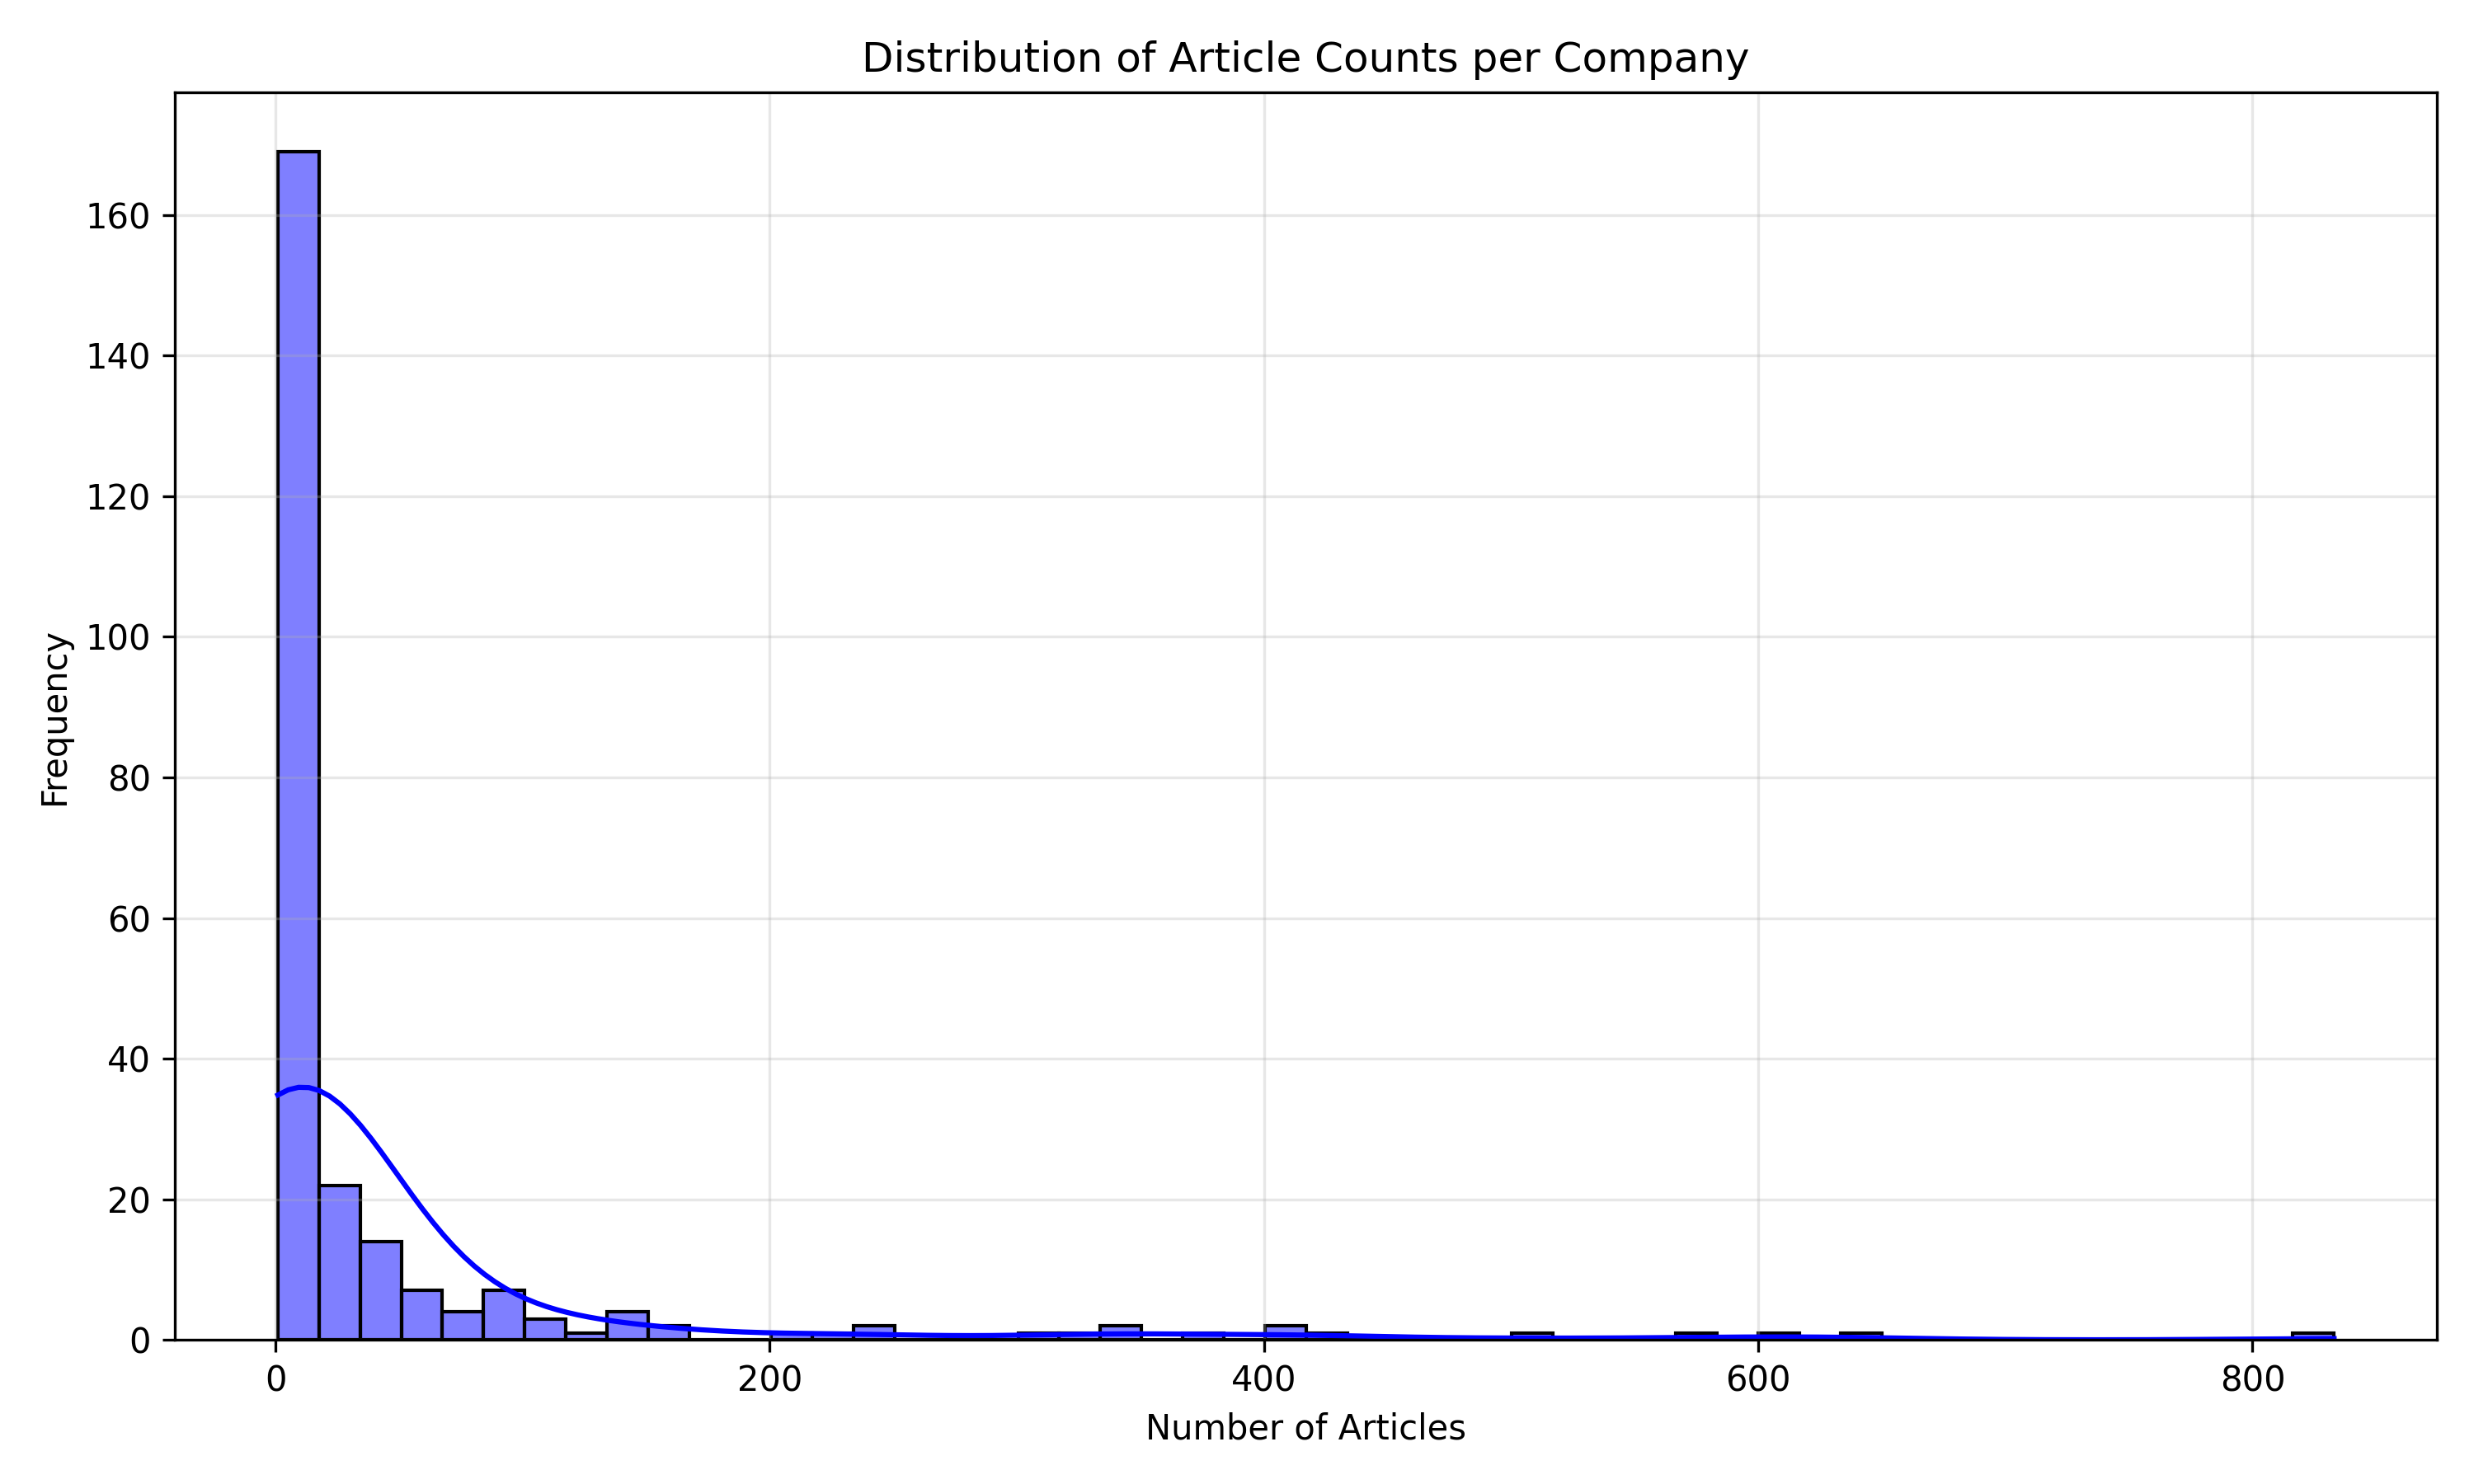
\includegraphics[width=\linewidth]{article_count_distribution.png}}
\caption{Distribution of article counts per company. The long tail motivates stratified sampling to avoid coverage-driven bias.}
\label{fig:article_count_distribution}
\end{figure}

\begin{figure}[htbp]
\centerline{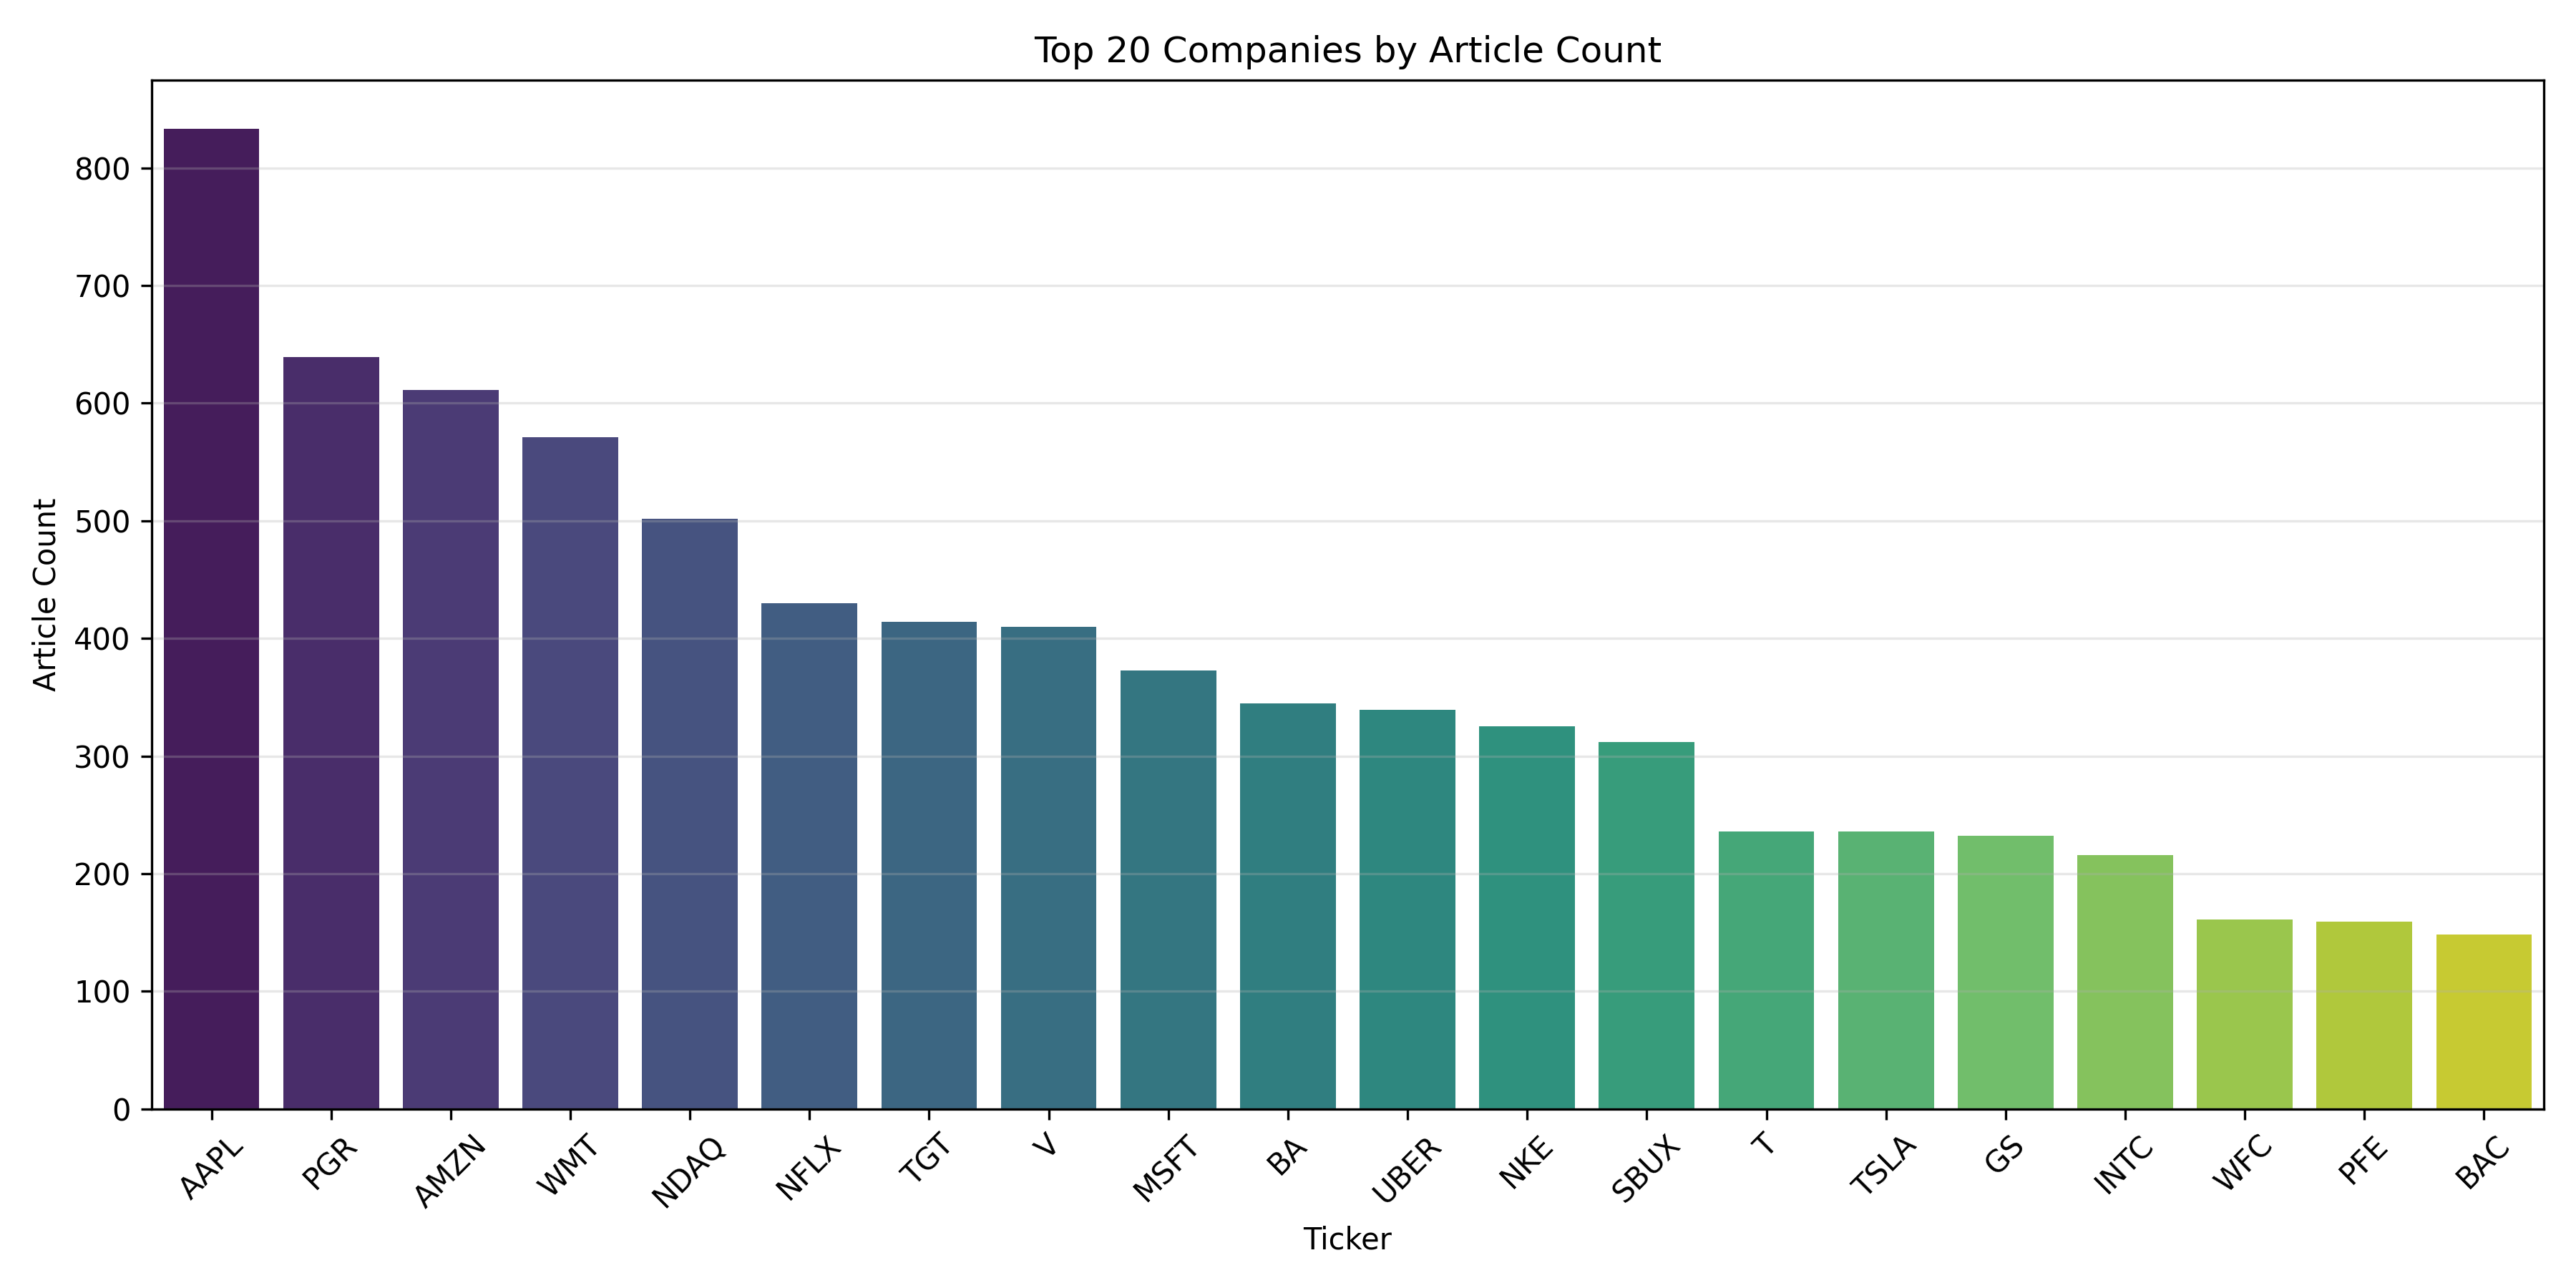
\includegraphics[width=\linewidth]{top_20_articles.png}}
\caption{Top 20 firms by article count in the retained sample.}
\label{fig:top20_articles}
\end{figure}

\subsection{Relevance Filtering and Annotation}
Keyword matching is not enough for firm targeting (e.g., ``Apple'' is not always the company). We therefore apply a two-stage relevance pipeline: (i) title-based pre-filtering that retains only articles with the company name in the title (company names, not tickers), and (ii) a supervised relevance classifier trained on manual annotations. The held-out test set for manual annotation is kept completely separate from training.

Our base classifier is DeBERTa-v3 fine-tuned for binary classification using article titles. The first model, trained on 750 labeled articles, achieved high recall but insufficient precision. We then expanded the training data via semi-supervised mining: running the model on a large unlabeled pool and adding only high-confidence predictions ($p_{rel} \ge 0.92$ for relevant, $p_{rel} \le 0.05$ for irrelevant). This expanded set increases precision and reduces false positives. An ensemble of model variants further improves precision, and the operating threshold is selected via a sweep to meet a target of precision $\ge 0.90$.

\subsection{Stance Scoring}
Stance is computed using the NewsMTSC model for target-dependent stance. For each qualifying article we obtain probabilities for positive, negative, and neutral stance. The baseline specification retains only high-confidence outputs (prob >= 0.9), and we report sensitivity to lower thresholds (0.6 and 0.0). Daily firm-level stance is the average across articles on that day:
\begin{equation}
\text{stance}_{i,t} = \frac{1}{N_{i,t}} \sum_{a \in A_{i,t}} (p^{+}_{a} - p^{-}_{a})
\end{equation}
where $A_{i,t}$ is the set of high-confidence articles for firm $i$ on day $t$ and $N_{i,t}$ is the count. We also construct article volume and coverage mix covariates to separate tone shifts from coverage shifts.

\subsection{Market Alignment and Controls}
The stance series is aligned to firm-day market outcomes: daily returns, S\&P 500 index returns, and VIX. We also log-normalize article volume in regressions. This alignment yields the panel used across the RQ1--RQ3 specifications.

\section{Methodology}
This section groups the empirical strategy into three layers: (i) structural shifts around the 2020 shock, (ii) stance-return linkage, and (iii) time-series dynamics and event studies.

\subsection{RQ1: Stance Shift Around the 2020 Shock}
We test for a structural shift in stance using a pre/post specification with firm fixed effects:
\begin{equation}
\text{stance}_{i,t} = \alpha_i + \beta \cdot Post_t + \gamma' X_{i,t} + \varepsilon_{i,t}
\end{equation}
where $Post_t$ equals 1 after January 2020 (post period: 2020--2025; pre: 2015--2019) and $X_{i,t}$ includes article volume and VIX. If pre-period means are not comparable, we implement Synthetic Control DiD (SCDiD) or use an interrupted time-series specification with level and trend shifts.

\subsection{RQ2: Returns Shift Around the 2020 Shock}
The returns analogue mirrors the stance regression, with returns as the outcome and market controls added:
\begin{equation}
\text{return}_{i,t} = \alpha_i + \beta\,\text{Post}_t + \gamma' X_{i,t} + \varepsilon_{i,t}
\end{equation}
where $X_{i,t}$ includes index returns and VIX to absorb market-wide shocks.

\subsection{RQ3: Stance-Return Linkage}
We test the direct stance-return relationship using next-day returns:
\begin{equation}
\text{return}_{i,t+1} = \alpha_i + \beta\,\text{stance}_{i,t} + \gamma' X_{i,t} + \varepsilon_{i,t}
\end{equation}
To test whether the stance-to-return sensitivity changes post-2020, we use a triple interaction:
\begin{equation}
\begin{aligned}
\text{return}_{i,t} &= \alpha_i + \beta\,\text{Post}_t + \gamma\,\text{stance}_{i,t} \\
&\quad + \delta(\text{Post}_t \times \text{stance}_{i,t}) + \theta X_{i,t} + \varepsilon_{i,t}
\end{aligned}
\end{equation}
where the interaction $\text{Post}_t \times \text{stance}_{i,t}$ captures post-shock amplification of the stance-return channel.

\subsection{Time-Series Dynamics and Event Studies}
We estimate VARs on (stance, returns) to capture bidirectional dynamics and compute impulse response functions. Granger causality tests evaluate whether past stance improves return forecasts beyond past returns, and whether the reverse also holds. We also test for autocorrelation in stance using ARIMA models, which motivates lagged stance controls.

As a non-parametric check, we run event studies around large stance jumps (e.g., >2 SD from a rolling mean) and compute abnormal returns in short windows around those events.

\subsection{Robustness and Sensitivity}
We perform numerous robustness checks: alternative stance aggregation (median, winsorized means), different confidence thresholds, exclusion of low-coverage firm-days, placebo pre/post cutoffs, and treatments that control for article topical composition. We also test sensitivity to training-test splits for the relevance classifier and manual annotation thresholds.

\section{Empirical Methodology}
We test the project's hypotheses in two escalating stages that follow the logic of
the research questions. The first stage asks whether the 2020 shock moved the
\emph{level} of two firm-level series---media stance (RQ1) and stock returns
(RQ2). This is a static question and is answered with fixed-effects panel
regressions. The second stage asks the sharper question behind RQ3: whether the
shock changed the \emph{dynamic} relationship between the two series, that is,
whether past stance began to forecast returns after the break. This is a
time-series question and is answered with a vector autoregression (VAR) and a
Granger-causality framework. The two stages require different estimators, which
we specify in turn. So that the argument stays readable, the construction and
quality auditing of the underlying panel are summarized at a high level here and
reported firm-by-firm in the Appendix.

\subsection{Panel Regression Design}
The unit of analysis is the firm--day pair $(i,t)$. For each scored article $a$ of
firm $i$ published on date $t$, the NewsMTSC model returns a probability triple
$(p_a^{+},p_a^{-},p_a^{0})$ over positive, negative, and neutral stance toward the
target firm. We collapse this into a signed article stance
$s_a = p_a^{+}-p_a^{-}\in[-1,1]$, which is large in magnitude only when the model
is confident and one-sided, and average it into the firm--day media stance
\begin{equation}
\text{bias}_{it} = \frac{1}{|\mathcal{A}_{it}|}\sum_{a\in\mathcal{A}_{it}} s_a,
\end{equation}
where $\mathcal{A}_{it}$ is the set of qualifying articles for firm $i$ on day
$t$. The returns outcome is the firm--day simple return
$\text{return}_{it}=(P_{it}-P_{i,t-1})/P_{i,t-1}$ from adjusted close prices. The
treatment common to both questions is the post-shock indicator
$\text{Post}_t=\mathbf{1}[\,t\ge\text{2020-01-01}\,]$, which splits the panel into a
pre-period (2015--2019) and a post-period (2020--2025).

The choice of controls follows directly from what could otherwise masquerade as a
post-2020 effect. For RQ1 we include firm--day article volume
$\text{vol}_{it}=|\mathcal{A}_{it}|$, because averaging a noisy stance signal over
more articles mechanically pulls the mean toward zero; holding volume fixed
separates a genuine change in tone from a change in coverage. For RQ2 we include
the contemporaneous S\&P~500 index return $\text{sp500\_return}_t$ to absorb the
market-wide drift and the volatility index $\text{vix}_t$ to absorb common
volatility regimes; without them the post indicator would merely re-estimate the
average market path on each side of 2020 rather than the firm-specific component
of interest.

RQ1 is estimated with a two-way fixed-effects specification,
\begin{equation}
\text{bias}_{it} = \alpha_i + \delta_t + \beta\,\text{Post}_t
+ \gamma\,\text{vol}_{it} + \varepsilon_{it},
\label{eq:rq1twfe}
\end{equation}
where the firm effects $\alpha_i$ absorb every time-invariant firm
characteristic and the daily effects $\delta_t$ absorb every firm-invariant
daily shock. With both present, $\beta$ identifies only the idiosyncratic
within-firm shift in stance after 2020 that is orthogonal to common daily
movements. RQ2 mirrors this design with entity (firm) effects and the two market
controls,
\begin{equation}
\text{return}_{it} = \alpha_i + \beta\,\text{Post}_t
+ \gamma_1\,\text{sp500\_return}_t + \gamma_2\,\text{vix}_t + \varepsilon_{it}.
\label{eq:rq2fe}
\end{equation}

Both models are estimated by the within (Mundlak) transformation: each variable
is demeaned by its firm and, for RQ1, time means, and OLS is applied to the
transformed data,
$\hat{\theta}=(\tilde{X}^{\top}\tilde{X})^{-1}\tilde{X}^{\top}\tilde{y}$. This is
algebraically identical to dummy-variable OLS but avoids storing thousands of
fixed-effect columns. Inference uses heteroscedasticity-robust HC1 standard
errors, and because firms share common trading-day shocks we additionally report
day-clustered standard errors for RQ1, which are robust to arbitrary cross-firm
correlation within a trading day and are our preferred uncertainty estimate for
the static model.

\subsection{Dynamic Time-Series Design}
The regressions above identify shifts in the \emph{level} of each series but are,
by construction, silent on the relationship \emph{between} them over time. The
question behind RQ3---did the 2020 shock turn media stance into a leading
indicator of returns---is inherently dynamic, so we move to a vector
autoregression. For a firm with endogenous vector
$\mathbf{y}_t=(\Delta\text{bias}_t,\,r_t)^{\top}$, where $\Delta\text{bias}_t$ is
the first difference of the weekly bias index and $r_t$ is the weekly log return,
a reduced-form VAR of order $p$ is
\begin{equation}
\mathbf{y}_t = \mathbf{c} + \sum_{\ell=1}^{p}\mathbf{A}_\ell\,\mathbf{y}_{t-\ell}
+ \mathbf{u}_t,\qquad \mathbf{A}_\ell\in\R^{2\times2}.
\label{eq:var}
\end{equation}
The off-diagonal entries of the $\mathbf{A}_\ell$ carry the cross-dynamics: a
nonzero $(2,1)$ entry means past stance moves current returns, and a nonzero
$(1,2)$ entry means the reverse. The VAR is the minimal model that treats both
variables as endogenous and lets the data, rather than an a priori ordering,
reveal the direction of predictability.

\paragraph{From articles to a modeling panel.} Reaching a series that can be fed
to Eq.~\eqref{eq:var} requires several preparatory steps, each of which is
audited firm-by-firm in the Appendix and summarized here. A data-inventory pass
(Appendix~\ref{app:inventory}) shows that daily firm-level stance is too sparse
for several firms, so we aggregate to ISO weeks; this yields near-complete
coverage (median $99.8\%$ of weeks) for sixteen well-covered firms while
retaining roughly $522$ weekly observations each. Short coverage gaps are
forward-filled and medium gaps linearly interpolated, with long gaps left missing
(Appendix~\ref{app:gaps}); both an imputed and an observed-only series are kept so
that every downstream test can be re-run to confirm results are not artifacts of
imputation. Returns are constructed as Monday-anchored weekly log returns and
aligned to the bias index (Appendix~\ref{app:returns}).

\paragraph{Stationarity dictates the specification.} A VAR in levels is valid
only if the series are stationary or jointly cointegrated; otherwise the
regression is spurious. Combining the Augmented Dickey--Fuller test (null: unit
root) with the KPSS test (null: stationarity), weekly log returns are
stationary, $I(0)$, for essentially every firm, whereas the bias index is
predominantly $I(1)$ or break-driven in levels but $I(0)$ in first differences
(Appendix~\ref{app:stationarity}, illustrated in Fig.~\ref{fig:stat}). This is
why Eq.~\eqref{eq:var} is specified on $(\Delta\text{bias}_t,\,r_t)$ rather than
on the levels. A Johansen trace test finds a cointegrating relation for only one
firm, confirming that for the common $(\,I(1),I(0)\,)$ case a differenced VAR,
not a VECM, is correct.

\begin{figure}[!t]
\centerline{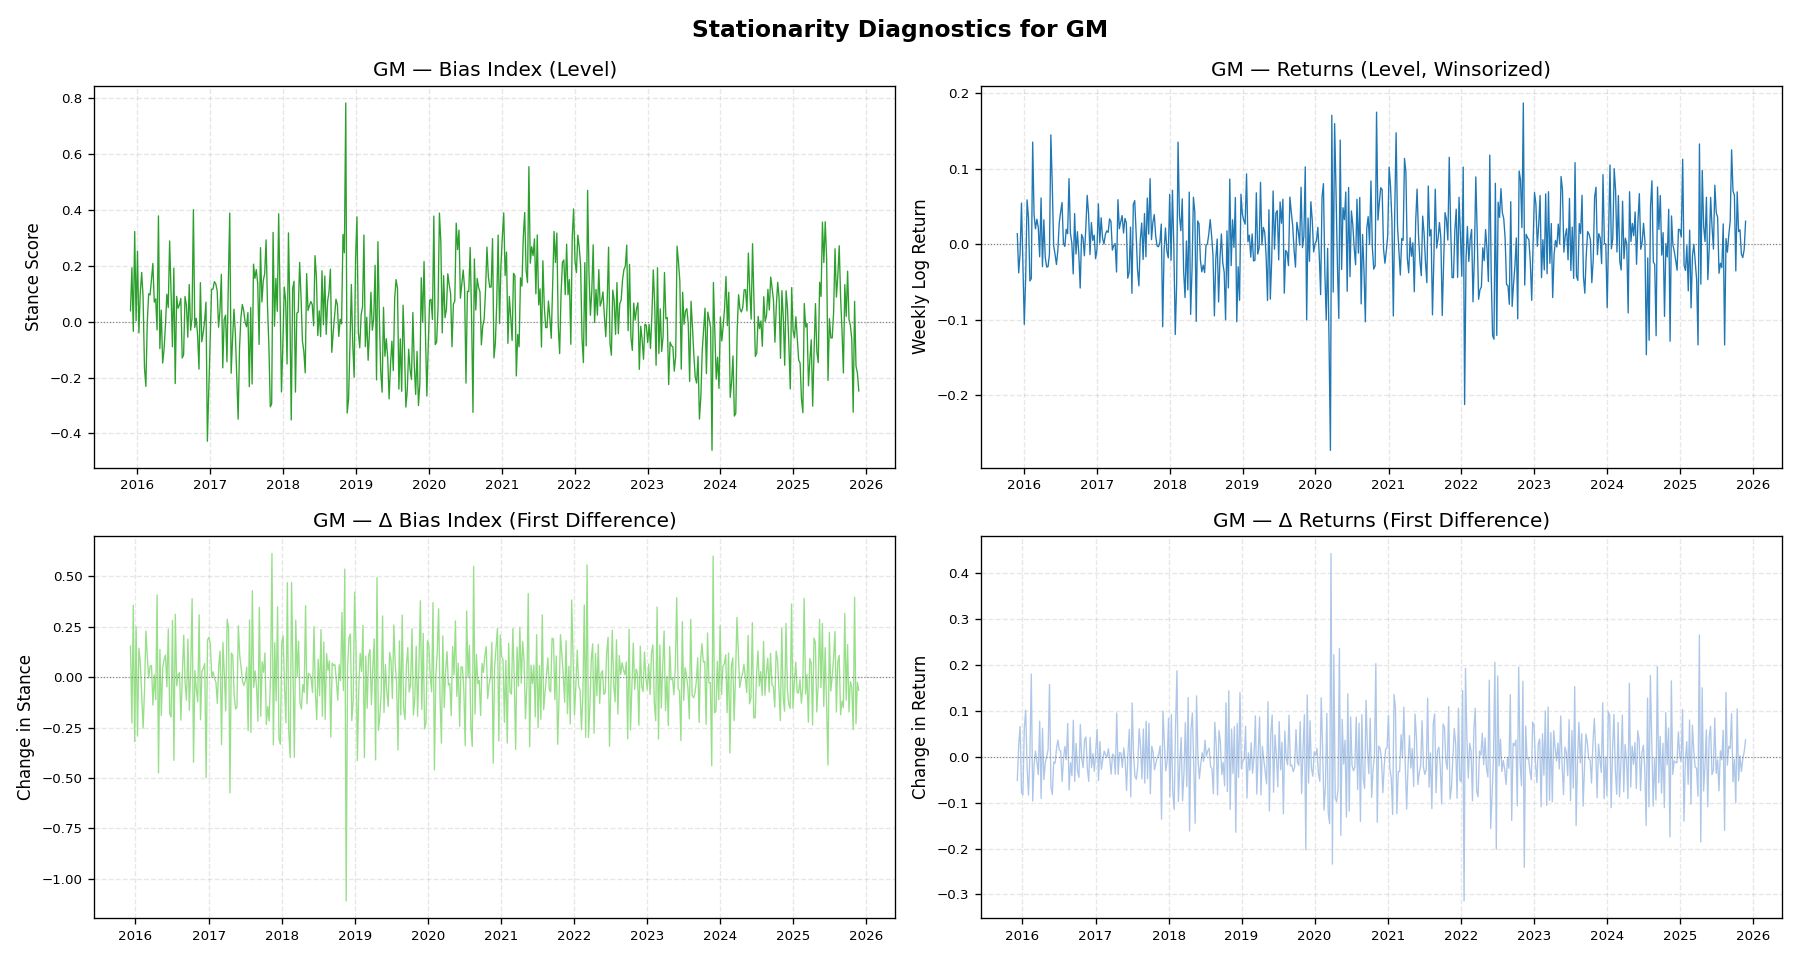
\includegraphics[width=\columnwidth]{fig_stationarity_GM.png}}
\caption{Stationarity diagnostics for a representative firm (GM): the bias index
and weekly return in levels (left) and first differences (right), with the ADF
and KPSS verdicts that drive the integration-order classification.}
\label{fig:stat}
\end{figure}

\paragraph{Lag order and stability.} For each firm the order $p$ is selected by
minimizing the Bayesian Information Criterion over $p=1,\dots,8$ (the BIC favors
parsimony; a floor of $p=1$ keeps the model dynamic), giving a modal choice of
$p=3$. Each fitted model is required to be stable---all roots of the companion
matrix outside the unit circle---and its residuals are screened for remaining
autocorrelation, normality, and ARCH effects (Appendix~\ref{app:varspec}). The
heavy tails and volatility clustering typical of financial data appear as
expected and motivate the robust inference used next.

\paragraph{Dating the regime change.} Because the central hypothesis concerns a
regime change, we date breaks empirically rather than imposing the calendar. A
Bai--Perron procedure, solved by dynamic programming for a single mean-shift
change point, locates the largest structural break in each weekly series; the
bias-index break date defines the pre/post split used for the subsample
causality tests (Appendix~\ref{app:breaks}, Figs.~\ref{fig:breakV}
and~\ref{fig:breakWFC}). Some breaks cluster near the COVID window while others
are firm-specific, which is itself evidence that a single imposed 2020 dummy
would be too blunt.

\begin{figure}[!t]
\centerline{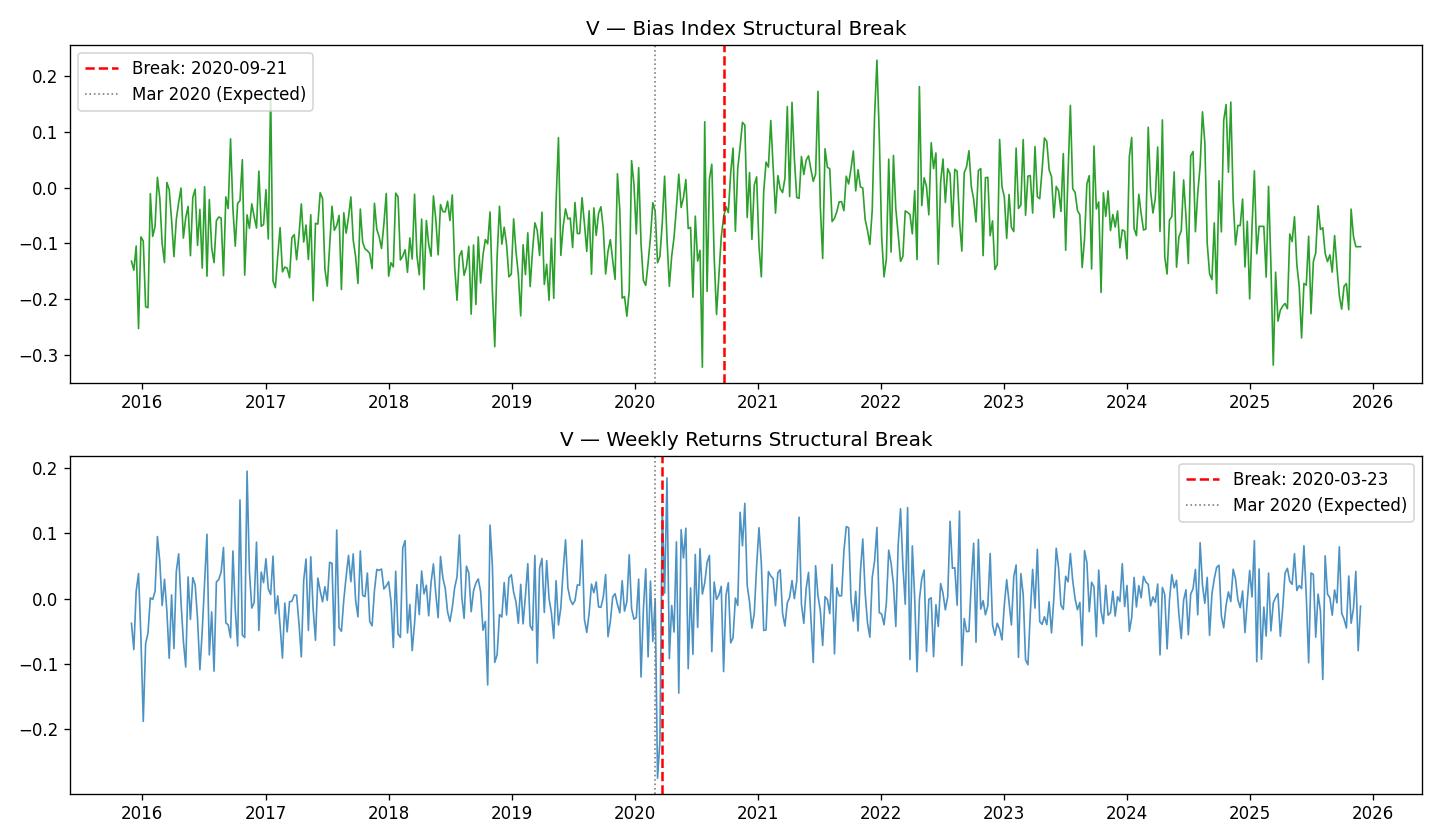
\includegraphics[width=\columnwidth]{fig_breaks_V.png}}
\caption{Data-driven structural breaks for Visa (V): the return break
(2020-03-23) coincides with the COVID crash, while the bias break (2020-09-21)
lags it.}
\label{fig:breakV}
\end{figure}

\paragraph{Granger causality.} Stance Granger-causes returns if the lagged
stance coefficients are jointly nonzero in the return equation, i.e.\ $H_0:
a^{(2,1)}_1=\dots=a^{(2,1)}_p=0$ is rejected. We test each direction with a joint
Wald ($F$) test on an OLS regression of each variable on $p$ lags of both,
using Newey--West HAC-robust standard errors ($\texttt{maxlags}=p$) to neutralize
the heteroscedasticity and autocorrelation found above. Firm-by-firm tests are
underpowered on a single short series, so we also pool the cross-section into a
panel VAR. Unobserved firm heterogeneity is removed with the
Arellano--Bover/Helmert transformation (forward mean-differencing),
\begin{equation}
\tilde{y}_{it} = c_{it}\Bigl(y_{it}-\tfrac{1}{T_{it}}\textstyle\sum_{s>t}y_{is}\Bigr),
\end{equation}
which subtracts the mean of all \emph{future} within-firm values and, unlike
ordinary demeaning, preserves orthogonality between the transformed variables and
the lagged regressors, avoiding the Nickell bias of dynamic fixed-effects panels.
The panel model additionally partials out the exogenous controls $\text{Post}_t$,
VIX, the S\&P~500 weekly log return, and the article count, so that any detected
causality cannot be attributed to market-wide volatility or coverage volume. It
is estimated by pooled OLS on the transformed, constant-free data with $p=3$ lags
and HAC-robust errors, over the full, pre-break, and post-break samples.

\begin{figure}[!t]
\centerline{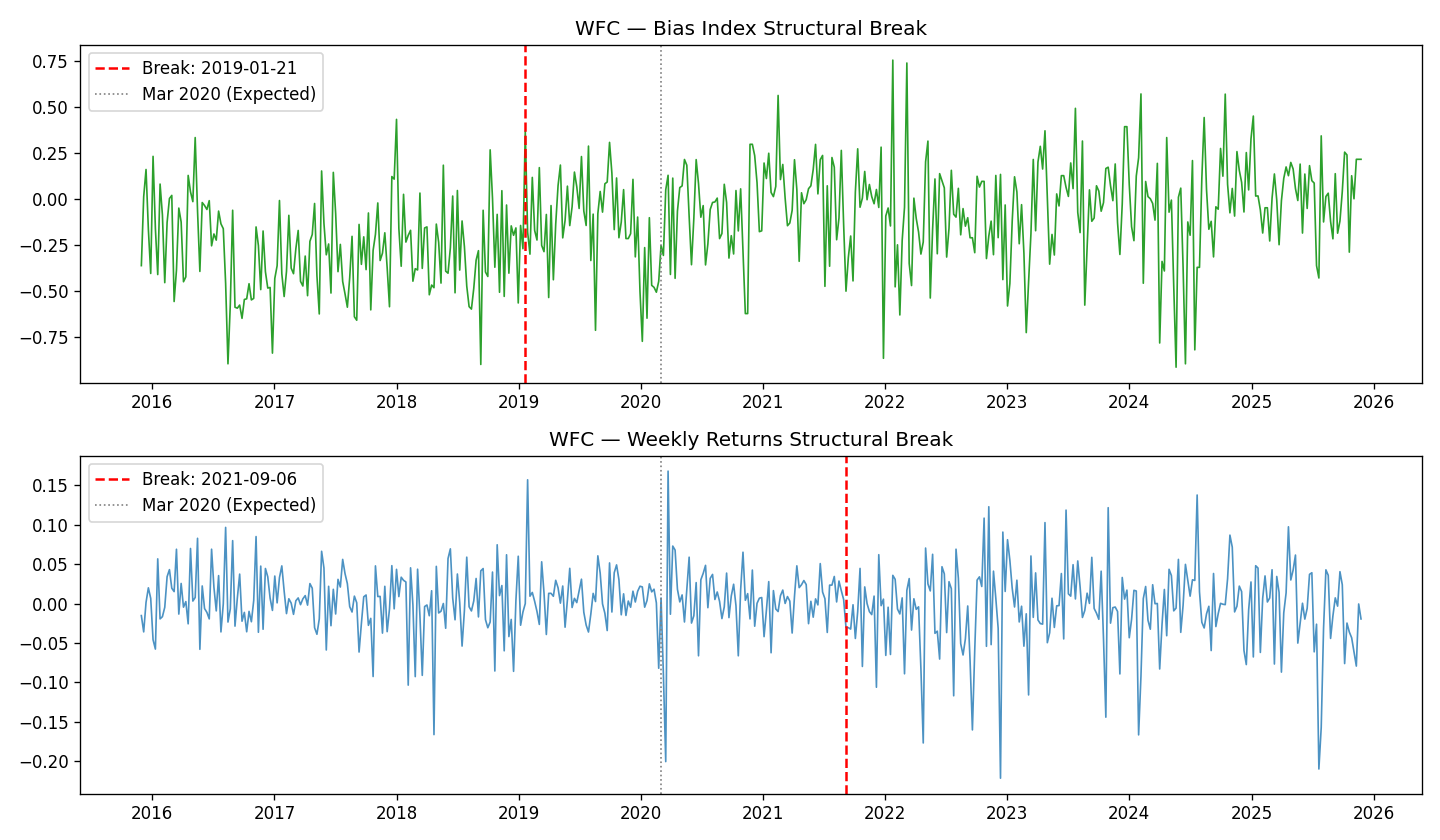
\includegraphics[width=\columnwidth]{fig_breaks_WFC.png}}
\caption{Structural breaks for Wells Fargo (WFC), the one firm with a
cointegrating bias--return relation and significant full-sample causality.}
\label{fig:breakWFC}
\end{figure}

\section{Empirical Results}
\label{sec:results}
We report the static results first (RQ1, then RQ2) and then the dynamic results,
following the same order in which the methodology was built. Construction and
diagnostic tables are deferred to the Appendix; the tables here carry the
substantive findings.

\subsection{RQ1: Media Stance Around the Shock}
Table~\ref{tab:rq1} reports the two-way fixed-effects estimates. The post
coefficient is positive ($0.0141$) but statistically insignificant ($p=0.30$),
while article volume is strongly negative and highly significant, confirming that
heavier coverage is associated with more neutral average tone within a
firm--day. Day-clustered inference (SE $=0.0134$) is almost identical to the HC1
result, so within-day cross-firm dependence does not change the conclusion.

\begin{table}[!t]
\caption{RQ1: Two-Way Fixed-Effects Estimates of Media Stance ($\alpha_i+\delta_t$)}
\label{tab:rq1}
\centering
\small
\begin{tabular}{lrrr}
\toprule
Variable & Coef. & SE (HC1) & $p$-value \\
\midrule
Post            & $0.014130$  & $0.013623$ & $0.2996$ \\
Article Volume  & $-0.000970$ & $0.000076$ & $<0.0001$ \\
\midrule
\multicolumn{4}{l}{Firm--day obs. $n=63{,}200$; Firms $=26$; Days $=4{,}018$} \\
\multicolumn{4}{l}{Raw articles after filters $=690{,}586$; Within $R^2=0.0017$} \\
\bottomrule
\end{tabular}
\end{table}

The weak static coefficient is informative rather than a failure of the design.
An $F$-test of the $4{,}017$ daily fixed effects against a firm-only model is
jointly significant ($F=1.135$ versus a $5\%$ critical value of $1.038$,
$p=1.1\times10^{-8}$), so daily shocks absorb most of the temporal variation in
stance. That leaves the coarse stepwise $\text{Post}_t$ indicator with little
residual variation to explain, which both attenuates $\beta$ and keeps the within
$R^2$ small. To recover the timing the single step compresses, a monthly event
study with firm effects and month-relative dummies around January 2020
(reference month $m=-1$) is reported in Table~\ref{tab:rq1es}: pre-shock
coefficients are small and insignificant, consistent with parallel trends,
whereas the post-shock effect builds gradually, becomes significant from about
three months onward, peaks at $m=+12$ ($0.064$, $p<0.001$), and remains elevated
at $m=+24$. The 2020 effect is therefore a slow, persistent uplift rather than a
discrete jump, which is precisely why the static term is muted once daily effects
are absorbed. The estimator satisfies the Gauss--Markov conditions, with HC1 and
clustered errors correcting the heteroscedasticity and large-$n$ asymptotics
covering the non-normal residuals; the full diagnostic battery is in
Appendix~\ref{app:mlr}.

\begin{table}[!t]
\caption{RQ1: Selected Monthly Event-Study Coefficients (Firm FE)}
\label{tab:rq1es}
\centering
\small
\begin{tabular}{lrrrl}
\toprule
Month & Coef. & SE (HC1) & $p$-value & Phase \\
\midrule
$m=-12$ & $0.021692$ & $0.018045$ & $0.2293$ & pre-trend \\
$m=-6$  & $0.031757$ & $0.017201$ & $0.0649$ & pre-trend \\
$m=0$   & $0.031032$ & $0.018354$ & $0.0909$ & event \\
$m=+3$  & $0.042152$ & $0.019168$ & $0.0279$ & early post \\
$m=+6$  & $0.032197$ & $0.018248$ & $0.0777$ & mid post \\
$m=+12$ & $0.064054$ & $0.018797$ & $0.0007$ & persistent \\
$m=+24$ & $0.050394$ & $0.018705$ & $0.0071$ & long-run \\
\bottomrule
\end{tabular}
\end{table}

\subsection{RQ2: Returns Around the Shock}
The returns panel contains $62{,}667$ firm--day observations across $26$ firms
(2015-12-01 to 2025-11-24). Table~\ref{tab:rq2} reports the entity
fixed-effects estimates. Conditional on the index return and VIX, the post-period
shift in daily firm returns is negative and marginally significant
($-0.000344$, $p=0.045$), about $-0.034\%$ per day. The market return loads near
unity and highly significantly, as expected for large-cap constituents, while VIX
is insignificant once the index return is included. The contrast with RQ1 is the
substantive payoff: media stance shows a slow post-2020 uplift while raw returns
show only a faint downward mean shift, which motivates asking not whether each
series shifts in level but whether the relationship between them changed.

\begin{table}[!t]
\caption{RQ2: Entity Fixed-Effects Estimates of Daily Returns (HC1 Robust SE)}
\label{tab:rq2}
\centering
\small
\begin{tabular}{lrrr}
\toprule
Variable & Coef. & SE (HC1) & $p$-value \\
\midrule
Post           & $-0.000344$ & $0.000172$ & $0.0451$ \\
S\&P 500 Return& $1.127576$  & $0.010982$ & $<0.0001$ \\
VIX            & $-0.000001$ & $0.000020$ & $0.9654$ \\
\bottomrule
\end{tabular}
\end{table}

\subsection{Dynamic Linkage: Granger Causality}
At the firm level, full-sample causality is sparse, as expected if the
relationship is regime-dependent: stance Granger-causes returns for Wells Fargo
($p=0.023$) and weakly for Morgan Stanley ($p=0.058$), and the reverse direction
is significant for Goldman Sachs ($p=0.012$); the remaining firms show no
significant direction (Appendix~\ref{app:granger}). The informative test splits
each firm at its empirical bias break. Several firms that are quiet in the full
sample show post-break causality absent pre-break---Wells Fargo
(bias$\to$returns $p=0.013$ post versus $0.345$ pre) and Morgan Stanley
(bias$\to$returns $p=0.052$ post) are the clearest---with feedback emerging
post-break for Boeing, Goldman Sachs, and Morgan Stanley. This pre/post asymmetry
is the firm-level analogue of the structural shift the regressions probe: the
link is not constant but switches on after the break for a subset of firms.

Pooling the cross-section into the panel VAR buys statistical power, yet
Table~\ref{tab:panelvar} shows that neither Granger direction is significant in
any subsample once VIX, the index return, and article volume are controlled.

\begin{table}[!t]
\caption{Panel VAR Granger Causality (15 firms, Helmert-transformed, HAC)}
\label{tab:panelvar}
\centering
\small
\begin{tabular}{lrrr}
\toprule
Sample & $N$ & Bias$\to$Ret & Ret$\to$Bias \\
\midrule
Full        & $7493$ & $0.976$ & $0.200$ \\
Pre-break   & $4168$ & $0.245$ & $0.801$ \\
Post-break  & $3265$ & $0.617$ & $0.187$ \\
\bottomrule
\end{tabular}
\end{table}

\subsection{Synthesis}
The three results compose a coherent picture. Media stance toward large-cap firms
did shift after 2020, but as a gradual uplift rather than a discrete jump; firm
returns shifted only faintly once market factors are removed; and the dynamic
link between stance and returns, where it appears at all, switches on after the
firm-specific break for a handful of firms and does not aggregate into a
market-wide channel. The panel VAR is exactly the test that would manufacture a
spurious aggregate effect if the controls were omitted, and it declines to do so.
The honest conclusion is that the post-2020 media--market relationship is real but
heterogeneous and firm-specific, not a uniform regularity---a finding that the
staged design, from static panels to a controlled panel VAR, is built to deliver
credibly. We collect the construction and diagnostic detail underlying every
stage in the Appendix and discuss residual threats to this interpretation next.


\section{Identification, Validity, and Robustness}
We address three main threats. First, macro shocks may move both coverage and prices; we control with index returns and VIX. Second, article volume differs widely across firms; we include volume covariates and run trimmed samples. Third, parallel trends may not hold; we use pre-trend checks, placebo cutoffs, and SCDiD when needed.

Robustness checks include alternate stance thresholds (0.9, 0.6, 0.0), alternative aggregation (mean vs median), lagged stance controls, sector controls, and quantile regressions to test for tail effects in returns.

\section{Conclusion and Next Steps}
This draft provides a full narrative of the project to date: why the 2020 shock matters, how we build a target-dependent stance signal, and how we test for structural changes and market effects. Next steps include finalizing the firm panel, completing the relevance classifier evaluation, computing the daily stance series, and running the full RQ1--RQ3 specifications with robustness tables and figures.

\appendices

\section{Data Inventory and Coverage}
\label{app:inventory}
Table~\ref{tab:app_inventory} reports per-firm article coverage for the sixteen
firms carried into the weekly modeling panel. Daily coverage exceeds $100\%$ for
most firms (more than one article per trading day on average); the share of
zero-article days motivates the move to a weekly frequency, at which coverage is
near-complete. Netflix was audited but dropped at the gap stage
(weekly coverage $59.2\%$); the firm-level inventory of sparse names excluded at
this stage (e.g.\ MMM, AAPL, ETN, NDAQ, NKE, ORCL, PGR, TSLA, each below $30\%$
daily coverage) is omitted for brevity.

\begin{table}[!t]
\caption{Per-firm coverage in the modeling panel}
\label{tab:app_inventory}
\centering
\small
\begin{tabular}{lrrrr}
\toprule
Ticker & Articles & Daily Cov.\,(\%) & Zero Days\,(\%) & Weekly Cov.\,(\%) \\
\midrule
ABNB & 13{,}771  & 116.3 & 17.1 & 99.8 \\
AMZN & 50{,}366  & 135.4 & 3.3  & 100.2 \\
T    & 139{,}701 & 139.6 & 1.5  & 99.0 \\
BA   & 47{,}140  & 133.1 & 4.9  & 100.2 \\
BAC  & 7{,}976   & 95.7  & 31.7 & 99.8 \\
GM   & 22{,}914  & 126.2 & 9.9  & 100.2 \\
GS   & 16{,}775  & 118.8 & 15.2 & 100.0 \\
INTC & 22{,}056  & 124.6 & 11.0 & 100.2 \\
MCD  & 26{,}849  & 127.9 & 8.6  & 100.2 \\
MSFT & 52{,}245  & 136.0 & 2.9  & 100.2 \\
MS   & 54{,}487  & 139.0 & 0.7  & 100.2 \\
SBUX & 19{,}955  & 119.4 & 15.8 & 99.0 \\
UBER & 36{,}774  & 125.1 & 11.7 & 99.0 \\
V    & 77{,}290  & 138.8 & 2.1  & 98.6 \\
WMT  & 38{,}196  & 133.7 & 5.7  & 99.0 \\
WFC  & 8{,}774   & 78.4  & 44.7 & 97.2 \\
\bottomrule
\end{tabular}
\end{table}

\section{Gap Analysis and Imputation}
\label{app:gaps}
Weekly gaps are classified by length: Type~A (1--2 weeks) are forward-filled and
Type~B (3--8 weeks) linearly interpolated, while Type~C ($>8$ weeks) are left
missing. Across all firms only $58$ observations are imputed ($16$ forward-fill,
$42$ interpolation), and every firm clears the $\ge 60\%$ coverage threshold with
no gap exceeding eight weeks (Table~\ref{tab:app_gaps}). The coverage map for the
sparsest retained firm is shown in Fig.~\ref{fig:gap}.

\begin{table}[!t]
\caption{Weekly gap classification and imputation counts}
\label{tab:app_gaps}
\centering
\small
\begin{tabular}{lrrrrr}
\toprule
Ticker & Cov.\,(\%) & Gaps A & Gaps B & Longest & Imputed \\
\midrule
ABNB & 99.7  & 1 & 0 & 2 & 2 \\
AMZN & 100.0 & 0 & 0 & 0 & 0 \\
T    & 98.8  & 0 & 1 & 7 & 7 \\
BA   & 100.0 & 0 & 0 & 0 & 0 \\
BAC  & 99.7  & 2 & 0 & 1 & 2 \\
GM   & 100.0 & 0 & 0 & 0 & 0 \\
GS   & 99.8  & 1 & 0 & 1 & 1 \\
INTC & 100.0 & 0 & 0 & 0 & 0 \\
MCD  & 100.0 & 0 & 0 & 0 & 0 \\
MSFT & 100.0 & 0 & 0 & 0 & 0 \\
MS   & 100.0 & 0 & 0 & 0 & 0 \\
SBUX & 98.8  & 0 & 1 & 7 & 7 \\
UBER & 98.8  & 0 & 1 & 7 & 7 \\
V    & 98.4  & 1 & 1 & 7 & 9 \\
WMT  & 98.8  & 0 & 1 & 7 & 7 \\
WFC  & 97.2  & 9 & 1 & 7 & 16 \\
\bottomrule
\end{tabular}
\end{table}

\begin{figure}[!t]
\centerline{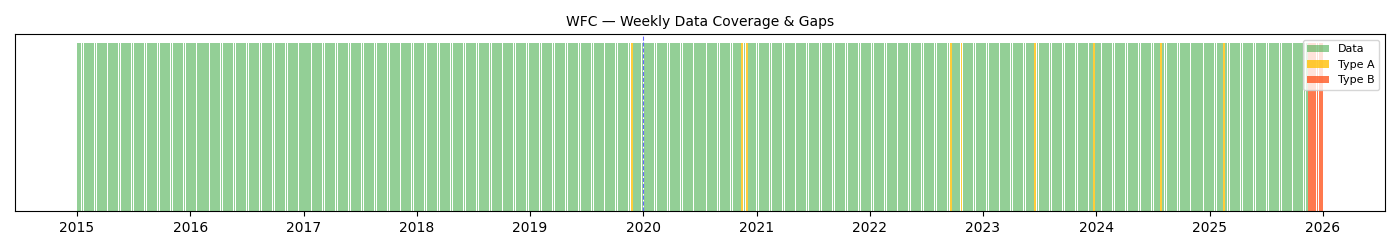
\includegraphics[width=\columnwidth]{fig_gap_WFC.png}}
\caption{Weekly coverage and gap map for Wells Fargo (WFC), the lowest-coverage
retained firm; it still clears the $\ge 60\%$ threshold after imputation.}
\label{fig:gap}
\end{figure}

\section{Returns Construction and Winsorization}
\label{app:returns}
Weekly log returns are computed from Monday-anchored ISO weeks and aligned to the
bias index (Table~\ref{tab:app_returns}). Extreme weekly moves ($>\pm15\%$)
cluster in the March 2020 crash window. Returns are winsorized at $\pm5$ standard
deviations from each firm's mean, with AT\&T (T) excluded from winsorization so
that its outlier behavior can be compared against the others.

\begin{table*}[!t]
\caption{Weekly log-return quality and winsorization (16 firms)}
\label{tab:app_returns}
\centering
\small
\begin{tabular}{lrrrrrrr}
\toprule
Ticker & Weeks & Mean & Std & Min & Max & Extreme ($>\!\pm15\%$) & Winsorized \\
\midrule
ABNB & 522 & $0.00265$  & $0.03562$ & $-0.1443$ & $0.1399$ & 0  & 0 \\
AMZN & 522 & $0.00235$  & $0.03230$ & $-0.1829$ & $0.1138$ & 1  & 1 \\
T    & 522 & $0.00147$  & $0.06861$ & $-0.4093$ & $0.3331$ & 18 & skipped \\
BA   & 522 & $-0.00046$ & $0.03924$ & $-0.2849$ & $0.1939$ & 4  & 1 \\
BAC  & 260 & $-0.00090$ & $0.06274$ & $-0.1815$ & $0.1896$ & 5  & 0 \\
GM   & 522 & $0.00503$  & $0.05559$ & $-0.2923$ & $0.1868$ & 6  & 1 \\
GS   & 522 & $0.00298$  & $0.03935$ & $-0.2026$ & $0.1322$ & 2  & 1 \\
INTC & 522 & $0.00224$  & $0.03584$ & $-0.1571$ & $0.1397$ & 1  & 0 \\
MCD  & 522 & $0.00251$  & $0.04381$ & $-0.2056$ & $0.2160$ & 5  & 0 \\
MSFT & 522 & $0.00209$  & $0.04499$ & $-0.2197$ & $0.1940$ & 6  & 0 \\
MS   & 522 & $0.00335$  & $0.04431$ & $-0.2955$ & $0.2533$ & 6  & 2 \\
SBUX & 522 & $0.00264$  & $0.04417$ & $-0.1883$ & $0.1934$ & 3  & 0 \\
UBER & 522 & $0.00250$  & $0.04123$ & $-0.2416$ & $0.2012$ & 4  & 1 \\
V    & 522 & $0.00154$  & $0.05526$ & $-0.2859$ & $0.1954$ & 6  & 1 \\
WMT  & 522 & $0.00154$  & $0.05526$ & $-0.2859$ & $0.1954$ & 6  & 1 \\
WFC  & 522 & $0.00012$  & $0.04667$ & $-0.2215$ & $0.1680$ & 10 & 0 \\
\bottomrule
\end{tabular}
\end{table*}

\section{Stationarity and Cointegration}
\label{app:stationarity}
Integration orders combine the ADF and KPSS verdicts on the levels and first
differences of each series (Table~\ref{tab:app_stat}). Returns are $I(0)$ almost
everywhere; the bias index is predominantly $I(1)$ or break-driven in levels.
A Johansen trace test detects cointegration only for Wells Fargo
(trace $=340.20$ at $r=0$ versus a $95\%$ critical value of $15.49$), which is the
single VECM candidate; for the common $(\,I(1),I(0)\,)$ pairing cointegration is
impossible, confirming the differenced VAR.

\begin{table}[!t]
\caption{Integration order of bias and return series}
\label{tab:app_stat}
\centering
\small
\begin{tabular}{lll}
\toprule
Ticker & (Bias, Return) & Note \\
\midrule
ABNB & $(I(1),I(0))$ & bias break-driven \\
AMZN & $(I(1),I(0))$ & \\
T    & $(I(1),I(0))$ & \\
BA   & $(I(0),I(1))$ & return break-driven \\
BAC  & $(I(1),I(0))$ & \\
GM   & $(I(0),I(0))$ & both stationary \\
GS   & $(I(1),I(0))$ & \\
INTC & $(I(1),I(0))$ & \\
MCD  & $(I(1),I(0))$ & \\
MSFT & $(I(1),I(0))$ & \\
MS   & $(I(1),I(0))$ & \\
SBUX & $(I(1),I(0))$ & \\
UBER & $(I(1),I(0))$ & \\
V    & $(I(1),I(0))$ & \\
WMT  & $(I(1),I(0))$ & \\
WFC  & $(I(1),I(1))$ & cointegrated (VECM) \\
\bottomrule
\end{tabular}
\end{table}

\section{VAR Lag Selection and Residual Diagnostics}
\label{app:varspec}
Lag orders are chosen by BIC over $p=1,\dots,8$; Table~\ref{tab:app_varspec}
reports the AIC and BIC choices, the selected order, and residual diagnostics.
Every selected model is stable (minimum companion root $>1$). The Portmanteau
test confirms adequate lag length for most firms, Jarque--Bera rejects normality
everywhere (heavy tails), and Engle's ARCH test flags volatility clustering in
several return residuals---together motivating the HAC-robust causality tests.
WMT is excluded from this specification pass.

\begin{table*}[!t]
\caption{VAR lag selection and residual diagnostics (15 firms)}
\label{tab:app_varspec}
\centering
\small
\begin{tabular}{lrrrrcrrrrr}
\toprule
Ticker & AIC & BIC & Chosen & $N$ & Stable & Min Root & Portm.\,$p$ & JB\,$p$ & ARCH(B)\,$p$ & ARCH(R)\,$p$ \\
\midrule
ABNB & 6 & 3 & 3 & 521 & \checkmark & 1.56 & 0.0553 & 0.0000 & 0.0264 & 0.0301 \\
AMZN & 7 & 2 & 2 & 521 & \checkmark & 1.99 & 0.0006 & 0.0000 & 0.1811 & 0.0000 \\
T    & 6 & 4 & 4 & 521 & \checkmark & 1.40 & 0.0985 & 0.0000 & 0.3270 & 0.8143 \\
BA   & 4 & 4 & 4 & 521 & \checkmark & 1.37 & 0.3284 & 0.0000 & 0.0784 & 0.0000 \\
BAC  & 4 & 1 & 1 & 259 & \checkmark & 2.02 & 0.0163 & 0.0000 & 0.0640 & 0.2924 \\
GM   & 7 & 3 & 3 & 521 & \checkmark & 1.55 & 0.0137 & 0.0000 & 0.0000 & 0.0003 \\
GS   & 8 & 5 & 5 & 521 & \checkmark & 1.28 & 0.0410 & 0.0000 & 0.5783 & 0.0007 \\
INTC & 8 & 2 & 2 & 521 & \checkmark & 1.80 & 0.0008 & 0.0000 & 0.1713 & 0.0000 \\
MCD  & 8 & 3 & 3 & 521 & \checkmark & 1.56 & 0.0003 & 0.0000 & 0.0002 & 0.0000 \\
MSFT & 8 & 3 & 3 & 521 & \checkmark & 1.65 & 0.0115 & 0.0000 & 0.0582 & 0.2155 \\
MS   & 7 & 3 & 3 & 521 & \checkmark & 1.53 & 0.0001 & 0.0000 & 0.6324 & 0.0000 \\
SBUX & 8 & 2 & 2 & 521 & \checkmark & 1.76 & 0.0035 & 0.0000 & 0.0378 & 0.0000 \\
UBER & 8 & 3 & 3 & 521 & \checkmark & 1.53 & 0.0220 & 0.0000 & 0.0000 & 0.0000 \\
V    & 8 & 3 & 3 & 521 & \checkmark & 1.65 & 0.0005 & 0.0000 & 0.0002 & 0.0000 \\
WFC  & 6 & 5 & 5 & 521 & \checkmark & 1.28 & 0.4343 & 0.0000 & 0.0340 & 0.0000 \\
\bottomrule
\end{tabular}
\end{table*}

\section{Structural Break Dates}
\label{app:breaks}
Bai--Perron single-break dates for each weekly series, with the resulting pre/post
observation counts, are reported in Table~\ref{tab:app_breaks}. The bias-index
break defines the subsample split for the causality tests. Examples are plotted in
Figs.~\ref{fig:breakV} and~\ref{fig:breakWFC}.

\begin{table}[!t]
\caption{Empirical structural break dates}
\label{tab:app_breaks}
\centering
\small
\begin{tabular}{lllrr}
\toprule
Ticker & Bias Break & Return Break & Pre & Post \\
\midrule
ABNB & 2022-05-23 & 2021-09-06 & 338 & 184 \\
AMZN & 2018-02-05 & 2022-01-03 & 114 & 408 \\
T    & 2022-05-02 & 2021-09-27 & 335 & 187 \\
BA   & 2024-01-08 & 2022-01-03 & 423 & 99  \\
BAC  & 2022-04-25 & 2022-12-26 & 72  & 188 \\
GM   & 2022-10-10 & 2017-10-30 & 358 & 164 \\
GS   & 2019-05-13 & 2021-11-22 & 180 & 342 \\
INTC & 2024-03-25 & 2023-03-20 & 434 & 88  \\
MCD  & 2022-03-28 & 2023-10-30 & 330 & 192 \\
MSFT & 2023-06-12 & 2021-09-27 & 393 & 129 \\
MS   & 2023-12-11 & 2023-10-30 & 419 & 103 \\
SBUX & 2021-11-08 & 2022-10-03 & 310 & 212 \\
UBER & 2018-04-02 & 2024-04-01 & 122 & 400 \\
V    & 2020-09-21 & 2020-03-23 & 251 & 271 \\
WMT  & 2024-07-22 & 2020-03-23 & 451 & 71  \\
WFC  & 2019-01-21 & 2021-09-06 & 164 & 358 \\
\bottomrule
\end{tabular}
\end{table}

\section{Firm-Level Granger Causality}
\label{app:granger}
Table~\ref{tab:app_granger} reports HAC ($p$-value) Granger tests for every firm,
in both directions, over the full sample and the pre/post subsamples defined by
the bias break. Stars denote $^{*}p<0.10$, $^{**}p<0.05$, $^{***}p<0.01$.

\begin{table*}[!t]
\caption{Firm-level Granger causality, full and subsample (HAC $p$-values)}
\label{tab:app_granger}
\centering
\small
\begin{tabular}{lrrrrrrr}
\toprule
 & & \multicolumn{2}{c}{Full} & \multicolumn{2}{c}{Pre-break} & \multicolumn{2}{c}{Post-break} \\
\cmidrule(lr){3-4}\cmidrule(lr){5-6}\cmidrule(lr){7-8}
Ticker & Lag & B$\to$R & R$\to$B & B$\to$R & R$\to$B & B$\to$R & R$\to$B \\
\midrule
ABNB & 3 & 0.992 & 0.877 & 0.667 & 0.690 & 0.629 & 0.623 \\
AMZN & 2 & 0.732 & 0.759 & 0.196 & 0.339 & 0.815 & 0.278 \\
T    & 4 & 0.947 & 0.345 & 0.207 & 0.571 & 0.122 & 0.348 \\
BA   & 4 & 0.232 & 0.295 & 0.196 & 0.775 & 0.543 & 0.014** \\
BAC  & 1 & 0.845 & 0.985 & 0.836 & 0.862 & 0.676 & 0.778 \\
GM   & 3 & 0.218 & 0.765 & 0.304 & 0.489 & 0.451 & 0.835 \\
GS   & 5 & 0.757 & 0.012** & 0.699 & 0.833 & 0.902 & 0.007*** \\
INTC & 2 & 0.872 & 0.305 & 0.479 & 0.158 & 0.173 & 0.696 \\
MCD  & 3 & 0.192 & 0.258 & 0.259 & 0.027** & 0.077* & 0.484 \\
MSFT & 3 & 0.680 & 0.134 & 0.137 & 0.234 & 0.309 & 0.477 \\
MS   & 3 & 0.058* & 0.193 & 0.119 & 0.313 & 0.052* & 0.016** \\
SBUX & 2 & 0.971 & 0.379 & 0.328 & 0.582 & 0.243 & 0.414 \\
UBER & 3 & 0.750 & 0.192 & 0.489 & 0.980 & 0.856 & 0.190 \\
V    & 3 & 0.981 & 0.174 & 0.873 & 0.157 & 0.827 & 0.629 \\
WFC  & 5 & 0.023** & 0.307 & 0.345 & 0.247 & 0.013** & 0.636 \\
\bottomrule
\end{tabular}
\end{table*}

\section{RQ1 Regression Diagnostics}
\label{app:mlr}
Table~\ref{tab:app_mlr} summarizes the classical-linear-model diagnostics for the
RQ1 two-way fixed-effects estimator. Orthogonality and conditioning are
satisfied; heteroscedasticity and non-normality are present and handled by the
HC1/clustered errors and large-sample asymptotics, respectively; collinearity is
negligible.

\begin{table}[!t]
\caption{RQ1 summary diagnostics}
\label{tab:app_mlr}
\centering
\small
\begin{tabular}{lrl}
\toprule
Test & Statistic & Implication \\
\midrule
Residual mean         & $-9.0\times10^{-19}$ & orthogonality OK \\
Condition number      & $157.46$ & numerically stable \\
Breusch--Pagan (LM)   & $190.25$ & heteroscedastic (HC1 used) \\
Jarque--Bera          & $4541.18$ & fat tails ($n$ large) \\
VIF (both regressors) & $\approx 1.00$ & no collinearity \\
Max pairwise corr.    & $0.0189$ & negligible \\
Durbin--Watson        & $1.673$ & mild autocorrelation \\
\bottomrule
\end{tabular}
\end{table}


\bibliographystyle{IEEEtran}
\begin{thebibliography}{99}
\bibitem{hamborg2021} F. Hamborg and K. Donnay, ``NewsMTSC: Target-dependent stance classification in news articles,'' EACL, 2021.
\bibitem{haroon2020} O. Haroon and S. A. Rizvi, ``COVID-19: Media coverage and financial markets behavior,'' Finance Research Letters, 2020.
\bibitem{blajer2024} M. Blajer-Golebiewska, A. Honecker, and K. Nowak, ``Investor sentiment response to COVID-19: A sectoral analysis,'' North American Journal of Economics and Finance, 2024.
\bibitem{news2024} ``News and markets in the time of COVID-19,'' Journal of Financial and Quantitative Analysis, 2024.
\bibitem{davis2020} S. Davis, S. Hansen, and C. Seminario, ``Firm-level risk exposures and stock returns in the wake of COVID-19,'' NBER, 2020.
\bibitem{costola2023} M. Costola, M. Nofer, O. Hinz, and L. Pelizzon, ``Machine learning sentiment analysis, COVID-19 news and stock market reactions,'' Research in International Business and Finance, 2023.
\bibitem{bai2023} Z. Bai, Q. Han, J. Pan, and R. Zhang, ``Financial market sentiment and returns,'' Finance Research Letters, 2023.
\bibitem{xu2024} H. Xu, ``News bias in financial journalists' social networks,'' Journal of Accounting Research, 2024.
\end{thebibliography}

\end{document}